%---------------
%╔═╗╔═╗╔╦╗╦ ╦╔═╗
%╚═╗║╣  ║ ║ ║╠═╝
%╚═╝╚═╝ ╩ ╚═╝╩
%---------------

% language setup
\newcommand{\docLanguage}{ngerman}
%\newcommand{\docLanguage}{english}

% DOCUMENT SETUP
\documentclass[12pt, oneside, a4paper, \docLanguage]{report}
\usepackage[left=3cm,
			right=2.5cm,
			top=2.5cm,
			bottom=2.5cm,
			includehead,
			includefoot]{geometry}

% line spacing
\usepackage{setspace}
\setstretch{1,25} % 15/12 --> 1.25

% encoding setup
% T1 font encoding for languages that use a latin alphabet
\usepackage[T1]{fontenc}

% enhanced input encoding handling - utf8 for äÄüÜöÖß...
\usepackage[utf8]{inputenc}

%de­fines Adobe Times Ro­man as de­fault text font
\usepackage{mathptmx}
\usepackage{times} % needed for acronym package

%PDF linking package
\usepackage[hidelinks]{hyperref}


% Language Setup
\usepackage[\docLanguage]{babel}
% after babel - set chapter string
\AtBeginDocument{\renewcommand{\chaptername}{}}

% language specific bibliography style
\usepackage[numbers, square]{natbib}
%\setcitestyle{square,aysep={},yysep={;}}
\usepackage{babelbib}
% bliographystyle setup
% babel specific: babplain, babplai3, babalpha, babunsrt, bababbrv, bababbr3
\bibliographystyle{babunsrt}


% enumeration
\usepackage{enumitem}
% tabular extension tabularx
\usepackage{tabularx}

% math packages
\usepackage{amsmath}
\usepackage{nicefrac}
\usepackage{amsthm}
\usepackage{amsbsy}
\usepackage{amssymb}
\usepackage{amsfonts}
%\usepackage{MnSymbol}


%special characters
\usepackage{amssymb}
\usepackage{upgreek,textgreek}

% acronym package
\usepackage[printonlyused, footnote]{acronym}

% breakable text in \seqsplit{}
\usepackage{seqsplit}

% \textmu
\usepackage{textcomp}

% package provides a way to compile sections of a document using the same preamble as the main document
\usepackage{subfiles}

% driver-independent color extension - used by listings,tabularx
\usepackage[usenames,dvipsnames,table,xcdraw]{xcolor}

% -- SYNTAX HIGHLIGHTING --
\usepackage{listings}
%% bash command line Syntax Highlighting
\lstdefinestyle{BASH_CMD}{ 
  columns=fullflexible,            % copy pasteable listings
  language=bash,
  basicstyle=\small\sffamily,
  basicstyle   = \small \ttfamily,
  keywordstyle = [1]\small \ttfamily,
  keywordstyle = [2]\small \ttfamily,
  commentstyle = \small \ttfamily,
  numbers=none,
  captionpos=b, 
  breaklines=true,
  numberstyle=\tiny,
  numbersep=3pt,
  frame=tlrb,
  columns=fullflexible,
  backgroundcolor=\color{white!20},
  linewidth=\linewidth,
  literate=                        % replace in code
     {Ö}{{\"O}}1
     {Ä}{{\"A}}1
     {Ü}{{\"U}}1
     {ß}{{\ss}}2
     {ü}{{\"u}}1
     {ä}{{\"a}}1
     {ö}{{\"o}}1
}
 % adds style BASH_CMD
%% Matlab Syntax Highlighting
\colorlet{keyword}{blue!100!black!80}
\colorlet{STD}{Lavender}
\colorlet{comment}{green!90!black!90}
\definecolor{mygreen}{rgb}{0,0.6,0}
\definecolor{mygray}{rgb}{0.5,0.5,0.5}
\definecolor{mymauve}{rgb}{0.58,0,0.82}


\lstdefinestyle{BASH_SCRIPT}{ 
  language     = bash,
  basicstyle   = \footnotesize \ttfamily,
  keywordstyle = [1]\color{keyword}\bfseries,
  keywordstyle = [2]\color{STD}\bfseries,
  commentstyle = \color{mygreen}\itshape,
  backgroundcolor=\color{white},   % choose the background color; you must add \usepackage{color} 
  columns=fullflexible,            % copy pasteable listings
                                   % or \usepackage{xcolor}
  basicstyle=\footnotesize,        % the size of the fonts that are used for the code
  breakatwhitespace=false,         % sets if automatic breaks should only happen at whitespace
  breaklines=true,                 % sets automatic line breaking
  captionpos=b,                    % sets the caption-position to bottom
  extendedchars=true,              % lets you use non-ASCII characters; for 8-bits encodings only,
                                   % does not work with UTF-8
  frame=single,                    % adds a frame around the code
  keepspaces=true,                 % keeps spaces in text, useful for keeping indentation of code
                                   % (possibly needs columns=flexible)
  numbers=left,                    % where to put the line-numbers; possible values are 
                                   % (none, left, right)
  numbersep=5pt,                   % how far the line-numbers are from the code
  numberstyle=\tiny\color{mygray}, % the style that is used for the line-numbers
  rulecolor=\color{black},         % if not set, the frame-color may be changed on line-breaks
                                   % within not-black text (e.g. comments (green here))
  showspaces=false,                % show spaces everywhere adding particular underscores; it
  	                               % overrides 'showstringspaces'
  showstringspaces=false,          % underline spaces within strings only
  showtabs=false,                  % show tabs within strings adding particular underscores
  stepnumber=1,                    % the step between two line-numbers. If it's 1, each line 
                                   % will be numbered
  stringstyle=\color{mymauve},     % string literal style
  tabsize=2,                       % sets default tabsize to 2 spaces
  title=\lstname,                  % set title name
  literate=                        % replace in code
     {Ö}{{\"O}}1 
     {Ä}{{\"A}}1 
     {Ü}{{\"U}}1 
     {ß}{{\ss}}2 
     {ü}{{\"u}}1 
     {ä}{{\"a}}1 
     {ö}{{\"o}}1 
     {â}{{\^{a}}}1 
     {Â}{{\^{A}}}1 
     {ç}{{\c{c}}}1 
     {Ç}{{\c{C}}}1 
     {ğ}{{\u{g}}}1 
     {Ğ}{{\u{G}}}1 
     {ı}{{\i}}1 
     {İ}{{\.{I}}}1 
     {ş}{{\c{s}}}1 
     {Ş}{{\c{S}}}1 
} % adds style BASH_SCRIPT
% Matlab Syntax Highlighting
\colorlet{keyword}{blue!100!black!80}
\colorlet{STD}{red}
\colorlet{comment}{green!90!black!90}
\definecolor{mygreen}{rgb}{0,0.6,0}
\definecolor{mygray}{rgb}{0.5,0.5,0.5}
\definecolor{mymauve}{rgb}{0.58,0,0.82}


\lstdefinestyle{LATEX}{ 
  language     = [LaTeX]{TeX},
  basicstyle   = \footnotesize \ttfamily,
  keywordstyle = [1]\color{keyword}\bfseries,
  keywordstyle = [2]\color{comment}\bfseries,
  commentstyle = \color{mygray}\itshape,
  %backgroundcolor=\color{white},   % choose the background color; you must add \usepackage{color} 
                                   % or \usepackage{xcolor}
  basicstyle=\footnotesize,        		   % the size of the fonts that are used for the code
  breakatwhitespace=false,         % sets if automatic breaks should only happen at whitespace
  columns=fullflexible,            % copy pasteable listings
  breaklines=true,                 % sets automatic line breaking
  captionpos=c,                    % sets the caption-position to bottom
  extendedchars=true,              % lets you use non-ASCII characters; for 8-bits encodings only,
                                   % does not work with UTF-8
  frame=single,                    % adds a frame around the code
  keepspaces=true,                 % keeps spaces in text, useful for keeping indentation of code
                                   % (possibly needs columns=flexible)
  numbers=left,                    % where to put the line-numbers; possible values are 
                                   % (none, left, right)
  numbersep=4pt,                   % how far the line-numbers are from the code
  numberstyle=\tiny\color{mygray}, % the style that is used for the line-numbers
  rulecolor=\color{black},         % if not set, the frame-color may be changed on line-breaks
                                   % within not-black text (e.g. comments (green here))
  showspaces=false,                % show spaces everywhere adding particular underscores; it
  	                               % overrides 'showstringspaces'
  showstringspaces=false,          % underline spaces within strings only
  showtabs=false,                  % show tabs within strings adding particular underscores
  stepnumber=1,                    % the step between two line-numbers. If it's 1, each line 
                                   % will be numbered
  stringstyle=\color{mymauve},     % string literal style
  tabsize=2,                       % sets default tabsize to 2 spaces
  title=\lstname,                  % set title name
  literate=                        % replace in code
     {Ö}{{\"O}}1 
     {Ä}{{\"A}}1 
     {Ü}{{\"U}}1 
     {ß}{{\ss}}2 
     {ü}{{\"u}}1 
     {ä}{{\"a}}1 
     {ö}{{\"o}}1 
     {â}{{\^{a}}}1 
     {Â}{{\^{A}}}1 
     {ç}{{\c{c}}}1 
     {Ç}{{\c{C}}}1 
     {ğ}{{\u{g}}}1 
     {Ğ}{{\u{G}}}1 
     {ı}{{\i}}1 
     {İ}{{\.{I}}}1 
     {ş}{{\c{s}}}1 
     {Ş}{{\c{S}}}1 
} % adds style LATEX
%% Matlab Syntax Highlighting
\colorlet{keyword}{blue!100!black!80}
\colorlet{STD}{Lavender}
\colorlet{comment}{green!90!black!90}
\definecolor{mygreen}{rgb}{0,0.6,0}
\definecolor{mygray}{rgb}{0.5,0.5,0.5}
\definecolor{mymauve}{rgb}{0.58,0,0.82}


\lstdefinestyle{MATLAB}{ 
  language     = Matlab,
  basicstyle   = \footnotesize \ttfamily,
  keywordstyle = [1]\color{keyword}\bfseries,
  keywordstyle = [2]\color{STD}\bfseries,
  commentstyle = \color{mygreen}\itshape,
  backgroundcolor=\color{white},   % choose the background color; you must add \usepackage{color} 
                                   % or \usepackage{xcolor}
  basicstyle=\footnotesize,        % the size of the fonts that are used for the code
  breakatwhitespace=false,         % sets if automatic breaks should only happen at whitespace
  columns=fullflexible,            % copy pasteable listings
  breaklines=false,                % sets automatic line breaking
  captionpos=c,                    % sets the caption-position to bottom
  extendedchars=true,              % lets you use non-ASCII characters; for 8-bits encodings only,
                                   % does not work with UTF-8
  frame=single,                    % adds a frame around the code
  keepspaces=true,                 % keeps spaces in text, useful for keeping indentation of code
                                   % (possibly needs columns=flexible)
  numbers=left,                    % where to put the line-numbers; possible values are 
                                   % (none, left, right)
  numbersep=5pt,                   % how far the line-numbers are from the code
  numberstyle=\tiny\color{mygray}, % the style that is used for the line-numbers
  rulecolor=\color{black},         % if not set, the frame-color may be changed on line-breaks
                                   % within not-black text (e.g. comments (green here))
  showspaces=false,                % show spaces everywhere adding particular underscores; it
  	                               % overrides 'showstringspaces'
  showstringspaces=false,          % underline spaces within strings only
  showtabs=false,                  % show tabs within strings adding particular underscores
  stepnumber=1,                    % the step between two line-numbers. If it's 1, each line 
                                   % will be numbered
  stringstyle=\color{mymauve},     % string literal style
  tabsize=2,                       % sets default tabsize to 2 spaces
  title=\lstname,                  % set title name
  literate=                        % replace in code
     {Ö}{{\"O}}1 
     {Ä}{{\"A}}1 
     {Ü}{{\"U}}1 
     {ß}{{\ss}}2 
     {ü}{{\"u}}1 
     {ä}{{\"a}}1 
     {ö}{{\"o}}1 
     {â}{{\^{a}}}1 
     {Â}{{\^{A}}}1 
     {ç}{{\c{c}}}1 
     {Ç}{{\c{C}}}1 
     {ğ}{{\u{g}}}1 
     {Ğ}{{\u{G}}}1 
     {ı}{{\i}}1 
     {İ}{{\.{I}}}1 
     {ş}{{\c{s}}}1 
     {Ş}{{\c{S}}}1 
} % adds style MATLAB
% Matlab Syntax Highlighting
\colorlet{keyword}{blue!100!black!80}
\colorlet{STD}{Lavender}
\colorlet{comment}{green!90!black!90}
\definecolor{mygreen}{rgb}{0,0.6,0}
\definecolor{mygray}{rgb}{0.5,0.5,0.5}
\definecolor{mymauve}{rgb}{0.58,0,0.82}


\lstdefinestyle{PYTHON}{ 
  language     = Python,
  basicstyle   = \footnotesize \ttfamily,
  keywordstyle = [1]\color{keyword}\bfseries,
  keywordstyle = [2]\color{STD}\bfseries,
  commentstyle = \color{mygreen}\itshape,
  backgroundcolor=\color{white},   % choose the background color; you must add \usepackage{color} 
                                   % or \usepackage{xcolor}
  basicstyle=\footnotesize,        % the size of the fonts that are used for the code
  columns=fullflexible,            % copy pasteable listings
  breakatwhitespace=false,         % sets if automatic breaks should only happen at whitespace
  breaklines=false,                % sets automatic line breaking
  captionpos=c,                    % sets the caption-position to bottom
  extendedchars=true,              % lets you use non-ASCII characters; for 8-bits encodings only,
                                   % does not work with UTF-8
  frame=single,                    % adds a frame around the code
  keepspaces=true,                 % keeps spaces in text, useful for keeping indentation of code
                                   % (possibly needs columns=flexible)
  numbers=left,                    % where to put the line-numbers; possible values are 
                                   % (none, left, right)
  numbersep=5pt,                   % how far the line-numbers are from the code
  numberstyle=\tiny\color{mygray}, % the style that is used for the line-numbers
  rulecolor=\color{black},         % if not set, the frame-color may be changed on line-breaks
                                   % within not-black text (e.g. comments (green here))
  showspaces=false,                % show spaces everywhere adding particular underscores; it
  	                               % overrides 'showstringspaces'
  showstringspaces=false,          % underline spaces within strings only
  showtabs=false,                  % show tabs within strings adding particular underscores
  stepnumber=1,                    % the step between two line-numbers. If it's 1, each line 
                                   % will be numbered
  stringstyle=\color{mymauve},     % string literal style
  tabsize=2,                       % sets default tabsize to 2 spaces
  title=\lstname,                  % set title name
  literate=                        % replace in code
     {Ö}{{\"O}}1 
     {Ä}{{\"A}}1 
     {Ü}{{\"U}}1 
     {ß}{{\ss}}2 
     {ü}{{\"u}}1 
     {ä}{{\"a}}1 
     {ö}{{\"o}}1 
     {â}{{\^{a}}}1 
     {Â}{{\^{A}}}1 
     {ç}{{\c{c}}}1 
     {Ç}{{\c{C}}}1 
     {ğ}{{\u{g}}}1 
     {Ğ}{{\u{G}}}1 
     {ı}{{\i}}1 
     {İ}{{\.{I}}}1 
     {ş}{{\c{s}}}1 
     {Ş}{{\c{S}}}1 
} % adds style PYTHON
%% Matlab Syntax Highlighting
\colorlet{keyword}{blue!100!black!80}
\colorlet{STD}{Lavender}
\colorlet{comment}{green!90!black!90}
\definecolor{mygreen}{rgb}{0,0.6,0}
\definecolor{mygray}{rgb}{0.5,0.5,0.5}
\definecolor{mymauve}{rgb}{0.58,0,0.82}


\lstdefinestyle{CPP}{ 
  language     = C++,
  basicstyle   = \footnotesize \ttfamily,
  keywordstyle = [1]\color{keyword}\bfseries,
  keywordstyle = [2]\color{STD}\bfseries,
  commentstyle = \color{mygreen}\itshape,
  backgroundcolor=\color{white},   % choose the background color; you must add \usepackage{color} 
                                   % or \usepackage{xcolor}
  columns=fullflexible,            % copy pasteable listings
  basicstyle=\footnotesize,        % the size of the fonts that are used for the code
  breakatwhitespace=false,         % sets if automatic breaks should only happen at whitespace
  breaklines=false,                % sets automatic line breaking
  captionpos=c,                    % sets the caption-position to bottom
  extendedchars=true,              % lets you use non-ASCII characters; for 8-bits encodings only,
                                   % does not work with UTF-8
  frame=single,                    % adds a frame around the code
  keepspaces=true,                 % keeps spaces in text, useful for keeping indentation of code
                                   % (possibly needs columns=flexible)
  numbers=left,                    % where to put the line-numbers; possible values are 
                                   % (none, left, right)
  numbersep=5pt,                   % how far the line-numbers are from the code
  numberstyle=\tiny\color{mygray}, % the style that is used for the line-numbers
  rulecolor=\color{black},         % if not set, the frame-color may be changed on line-breaks
                                   % within not-black text (e.g. comments (green here))
  showspaces=false,                % show spaces everywhere adding particular underscores; it
  	                               % overrides 'showstringspaces'
  showstringspaces=false,          % underline spaces within strings only
  showtabs=false,                  % show tabs within strings adding particular underscores
  stepnumber=1,                    % the step between two line-numbers. If it's 1, each line 
                                   % will be numbered
  stringstyle=\color{mymauve},     % string literal style
  tabsize=2,                       % sets default tabsize to 2 spaces
  title=\lstname,                  % set title name
  literate=                        % replace in code
     {Ö}{{\"O}}1 
     {Ä}{{\"A}}1 
     {Ü}{{\"U}}1 
     {ß}{{\ss}}2 
     {ü}{{\"u}}1 
     {ä}{{\"a}}1 
     {ö}{{\"o}}1 
     {â}{{\^{a}}}1 
     {Â}{{\^{A}}}1 
     {ç}{{\c{c}}}1 
     {Ç}{{\c{C}}}1 
     {ğ}{{\u{g}}}1 
     {Ğ}{{\u{G}}}1 
     {ı}{{\i}}1 
     {İ}{{\.{I}}}1 
     {ş}{{\c{s}}}1 
     {Ş}{{\c{S}}}1 
} % adds style CPP
%% Matlab Syntax Highlighting
\colorlet{keyword}{blue!100!black!80}
\colorlet{STD}{Lavender}
\colorlet{comment}{green!90!black!90}
\definecolor{mygreen}{rgb}{0,0.6,0}
\definecolor{mygray}{rgb}{0.5,0.5,0.5}
\definecolor{mymauve}{rgb}{0.58,0,0.82}


\lstdefinestyle{C}{ 
  language     = C,
  basicstyle   = \footnotesize \ttfamily,
  keywordstyle = [1]\color{keyword}\bfseries,
  keywordstyle = [2]\color{STD}\bfseries,
  commentstyle = \color{mygreen}\itshape,
  backgroundcolor=\color{white},   % choose the background color; you must add \usepackage{color} 
  columns=fullflexible,            % copy pasteable listings
                                   % or \usepackage{xcolor}
  basicstyle=\footnotesize,        % the size of the fonts that are used for the code
  breakatwhitespace=false,         % sets if automatic breaks should only happen at whitespace
  breaklines=false,                % sets automatic line breaking
  captionpos=c,                    % sets the caption-position to bottom
  extendedchars=true,              % lets you use non-ASCII characters; for 8-bits encodings only,
                                   % does not work with UTF-8
  frame=single,                    % adds a frame around the code
  keepspaces=true,                 % keeps spaces in text, useful for keeping indentation of code
                                   % (possibly needs columns=flexible)
  numbers=left,                    % where to put the line-numbers; possible values are 
                                   % (none, left, right)
  numbersep=5pt,                   % how far the line-numbers are from the code
  numberstyle=\tiny\color{mygray}, % the style that is used for the line-numbers
  rulecolor=\color{black},         % if not set, the frame-color may be changed on line-breaks
                                   % within not-black text (e.g. comments (green here))
  showspaces=false,                % show spaces everywhere adding particular underscores; it
  	                               % overrides 'showstringspaces'
  showstringspaces=false,          % underline spaces within strings only
  showtabs=false,                  % show tabs within strings adding particular underscores
  stepnumber=1,                    % the step between two line-numbers. If it's 1, each line 
                                   % will be numbered
  stringstyle=\color{mymauve},     % string literal style
  tabsize=2,                       % sets default tabsize to 2 spaces
  title=\lstname,                  % set title name
  literate=                        % replace in code
     {Ö}{{\"O}}1 
     {Ä}{{\"A}}1 
     {Ü}{{\"U}}1 
     {ß}{{\ss}}2 
     {ü}{{\"u}}1 
     {ä}{{\"a}}1 
     {ö}{{\"o}}1 
     {â}{{\^{a}}}1 
     {Â}{{\^{A}}}1 
     {ç}{{\c{c}}}1 
     {Ç}{{\c{C}}}1 
     {ğ}{{\u{g}}}1 
     {Ğ}{{\u{G}}}1 
     {ı}{{\i}}1 
     {İ}{{\.{I}}}1 
     {ş}{{\c{s}}}1 
     {Ş}{{\c{S}}}1 
} % adds style C
%% JSON Syntax Highlighting
\colorlet{keyword}{blue!100!black!80}
\colorlet{STD}{Lavender}
\colorlet{comment}{green!90!black!90}
\definecolor{mygreen}{rgb}{0,0.6,0}
\definecolor{mygray}{rgb}{0.5,0.5,0.5}
\definecolor{mymauve}{rgb}{0.58,0,0.82}

\newcommand\JSONnumbervaluestyle{\color{blue}}
\newcommand\JSONstringvaluestyle{\color{red}}

\newif\ifcolonfoundonthisline

\makeatletter

\lstdefinelanguage{json}
{
  showstringspaces    = false,
  keywords            = {false,true},
  alsoletter          = 0123456789.,
  morestring          = [s]{"}{"},
  morestring          = [s]{'}{'},
  stringstyle         = \ifcolonfoundonthisline\JSONstringvaluestyle\fi,
  MoreSelectCharTable =%
    \lst@DefSaveDef{`:}\colon@json{\processColon@json},
  basicstyle          = \ttfamily,
  keywordstyle        = \ttfamily\bfseries,
}

% flip the switch if a colon is found in Pmode
\newcommand\processColon@json{
  \colon@json%
  \ifnum\lst@mode=\lst@Pmode%
    \global\colonfoundonthislinetrue%
  \fi
}

\lst@AddToHook{Output}{%
  \ifcolonfoundonthisline%
    \ifnum\lst@mode=\lst@Pmode%
      \def\lst@thestyle{\JSONnumbervaluestyle}%
    \fi
  \fi
  %override by keyword style if a keyword is detected!
  \lsthk@DetectKeywords% 
}

% reset the switch at the end of line
\lst@AddToHook{EOL}%
  {\global\colonfoundonthislinefalse}

\makeatother



\lstdefinestyle{JSON}{ 
  language     = json,
  basicstyle   = \footnotesize \ttfamily,
  keywordstyle = [1]\color{keyword}\bfseries,
  keywordstyle = [2]\color{STD}\bfseries,
  commentstyle = \color{mygreen}\itshape,
  backgroundcolor=\color{white},   % choose the background color; you must add \usepackage{color} 
                                   % or \usepackage{xcolor}
  basicstyle=\footnotesize,        % the size of the fonts that are used for the code
  columns=fullflexible,            % copy pasteable listings
  breakatwhitespace=false,         % sets if automatic breaks should only happen at whitespace
  breaklines=false,                % sets automatic line breaking
  captionpos=c,                    % sets the caption-position to bottom
  extendedchars=true,              % lets you use non-ASCII characters; for 8-bits encodings only,
                                   % does not work with UTF-8
  frame=single,                    % adds a frame around the code
  keepspaces=true,                 % keeps spaces in text, useful for keeping indentation of code
                                   % (possibly needs columns=flexible)
  numbers=left,                    % where to put the line-numbers; possible values are 
                                   % (none, left, right)
  numbersep=5pt,                   % how far the line-numbers are from the code
  numberstyle=\tiny\color{mygray}, % the style that is used for the line-numbers
  rulecolor=\color{black},         % if not set, the frame-color may be changed on line-breaks
                                   % within not-black text (e.g. comments (green here))
  showspaces=false,                % show spaces everywhere adding particular underscores; it
  	                               % overrides 'showstringspaces'
  showstringspaces=false,          % underline spaces within strings only
  showtabs=false,                  % show tabs within strings adding particular underscores
  stepnumber=1,                    % the step between two line-numbers. If it's 1, each line 
                                   % will be numbered
  stringstyle=\color{mymauve},     % string literal style
  tabsize=2,                       % sets default tabsize to 2 spaces
  title=\lstname,                  % set title name
  literate=                        % replace in code
     {Ö}{{\"O}}1
     {Ä}{{\"A}}1
     {Ü}{{\"U}}1
     {ß}{{\ss}}2
     {ü}{{\"u}}1
     {ä}{{\"a}}1
     {ö}{{\"o}}1
} % adds style JSON

% HEADLINE CFG
\usepackage{fancyhdr} % Headers and footers
\usepackage{lastpage}
\usepackage{ifthen}
\setlength{\headheight}{1.5cm}
%\pagestyle{fancy} % All pages have headers and footers
% override plain page style for \part, \chapter or
% \maketitle, which implicit specifies plain page style
\fancypagestyle{plain} 
{
	\fancyhead[L]{}
	\fancyhead[C]{}
	\fancyhead[R]{}
	\fancyfoot[L]{}
	\fancyfoot[C]{\thepage}
	\fancyfoot[R]{}
}
% set list pagestyle
\fancypagestyle{preface} 
{
	\fancyhead[L]{}
	\fancyhead[C]{}
	\fancyhead[R]{}
	\fancyfoot[L]{}
	\fancyfoot[C]{\thepage}
	\fancyfoot[R]{}
}
% set default pagestyle
\fancypagestyle{default} 
{
	\fancyhead{} % Blank out the default header
	\fancyfoot{} % Blank out the default footer
	\fancyhead[L]{}
	\fancyhead[C]{}
	\fancyhead[R]{}
	\fancyfoot[L]{}
	\fancyfoot[C]{\thepage}
	\fancyfoot[R]{}
}
%\fancypagestyle{default} 
{
\fancyhead[L]{\ifthenelse{\isodd{\value{page}}}{\arabic{chapter} \rightmark}{}}
\fancyhead[R]{\thepage}
}

\renewcommand{\chaptermark}[1]{\markright{#1}{}}
\renewcommand{\sectionmark}[1]{\markright{#1}{}}
\renewcommand{\headrulewidth}{0pt}
\renewcommand{\footrulewidth}{0pt}

% PICTURE CFG
\usepackage{verbatim}
\usepackage{graphicx}
\usepackage{epstopdf}
\usepackage{caption}
\usepackage[list=true,listformat=simple]{subcaption}
% floating prevention packages
\usepackage{float}    % used with [H] positioning parameter
\usepackage{placeins} % \FloatBarrier
% tikz packages
\usepackage{tikz}
\usepackage{standalone}
\usepackage{pgfplots}


% include only specified tex files - uncommend here
\includeonly{preface/cover,
             preface/abstract,
             preface/tableofcontents,
             preface/listoffigures,
             preface/listoftables,
             preface/lstlistoflistings,
             appendix/bibliography}

%-------------------
%╔═╗╔╦╗╦═╗╦╔╗╔╔═╗╔═╗
%╚═╗ ║ ╠╦╝║║║║║ ╦╚═╗
%╚═╝ ╩ ╩╚═╩╝╚╝╚═╝╚═╝
%-------------------
\newcommand{\strLecture}{Signale, Systeme und Sensoren}
\newcommand{\strDate}{\today}
\newcommand{\strAuthorA}{D. Wollmann}
\newcommand{\strAuthorB}{V. Bratulescu}
%\newcommand{\strAuthorC}{C. Author}
\newcommand{\strAuthorAEmail}{da161wol@htwg-konstanz.de}
\newcommand{\strAuthorBEmail}{vl161bra@htwg-konstanz.de}
%\newcommand{\strAuthorCEmail}{cauthor@htwg-konstanz.de}
% Versuchsbeschreibung
\newcommand{\strTopic}{Kalibrierung von Digitalkameras}
\newcommand{\strAbstract}{

In diesem Versuch werden die Eigenschaften von digitalen Kameras untersucht. Dabei wird die Python Bibliothek OpenCV eingesetzt, um die Kamerasensoren zu kalibrieren. 
Ein Grauwertkeil wird mit einer digitalen Kamera aufgenommen und für jede Grauwertstufe den Mittelwert und die Standardabweichung berechnet. Als nächstes wird versucht die Auswirkungen des Dunkelstroms zu eliminieren. Dafür wird ein sogenanntes Dunkelbild erstellt, mit dem dann das Originalbild korrigiert wird. Außerdem gibt es noch das Problem, dass die Optik der Kamera die Helligkeit nicht gleichmäßig auf den Sensor überträgt und somit eine Vignettierung entsteht. Dafür wird ein Weißbild erstellt. Im letzten Teil der Aufgabe werden die Bilder auf funktionsuntüchtige Pixel, wie zum Beispiel hot, stuck und dead pixel untersucht.
}
% hyperref customization
\hypersetup{
	pdftitle     = {\strTopic}, % title
	pdfsubject   = {\strLecture}, % subject of the document
	pdfauthor    = {\strAuthorA, \strAuthorB}, % author
	pdfkeywords  = {}, % list of keywords
	pdfcreator   = {}, % creator of the document
	pdfproducer  = {}, % producer of the document
	colorlinks   = false, % false: boxed links; true: colored links
	linkcolor    = red, % color of internal links (change box color with linkbordercolor)
    citecolor    = green, % color of links to bibliography
    filecolor    = magenta, % color of file links
    urlcolor     = cyan, % color of external links
	%bookmarks    = true, % show bookmarks bar?
	unicode	     = true, % non-Latin characters in Acrobat’s bookmarks
	pdftoolbar   = true, % show Acrobat’s toolbar?
	pdfmenubar   = true, % show Acrobat’s menu?
    pdffitwindow = false, % window fit to page when opened
	pdfnewwindow = true % links in new PDF window
}

%-----------------------------------------
% ╔╗ ╔═╗╔═╗╦╔╗╔  ╔╦╗╔═╗╔═╗╦ ╦╔╦╗╔═╗╔╗╔╔╦╗
% ╠╩╗║╣ ║ ╦║║║║   ║║║ ║║  ║ ║║║║║╣ ║║║ ║
% ╚═╝╚═╝╚═╝╩╝╚╝  ═╩╝╚═╝╚═╝╚═╝╩ ╩╚═╝╝╚╝ ╩
%-----------------------------------------

\begin{document}
\pagenumbering{Roman}

\setcounter{section}{0}

\begin{titlepage}

\vspace*{-3.5cm}

\begin{flushleft}
\hspace*{-1cm} 
\includegraphics[width=15.7cm]{preface/htwg-logo}
\end{flushleft}

\vspace{1cm}

\begin{center}
	\large{
		\textbf{\strLecture} \\[2cm]
	}
	\Huge{
		\textbf{\strTopic} \\[2cm]
	}
	\Large{
		\textbf{\strAuthorA, \strAuthorB}} \\[3cm]
		%\textbf{\strAuthorA, \strAuthorB, \strAuthorC}} \\[3cm]
	\large{
		\textbf{} \\[2.3cm]
	}
	
	\large{
		\textbf{Konstanz, \strDate}
	}
\end{center}

\end{titlepage}
\thispagestyle{empty}




\begin{center}
{\Large \textbf{Zusammenfassung (Abstract)}}
\end{center}

\bigskip

\begin{center}
	\begin{tabular}{p{2.8cm}p{5cm}p{5cm}}
		Thema: & \multicolumn{2}{p{10cm}}{\raggedright\strTopic} \\
		 & & \\
		Autoren: & \strAuthorA & \href{mailto:\strAuthorAEmail}{\strAuthorAEmail} \\
		 & \strAuthorB & \href{mailto:\strAuthorBEmail}{\strAuthorBEmail} \\
		 & & \\
		Betreuer: & Prof. Dr. Matthias O. Franz & \href{mailto:mfranz@htwg-konstanz.de}{mfranz@htwg-konstanz.de} \\
		 &  Jürgen Keppler & \href{mailto:juergen.keppler@htwg-konstanz.de}{juergen.keppler@htwg-konstanz.de} \\
		 &  Martin Miller & \href{mailto:martin.miller@htwg-konstanz.de}{martin.miller@htwg-konstanz.de} \\
	\end{tabular}
\end{center}

\bigskip

\noindent
\strAbstract

\thispagestyle{lists}



\clearpage

%
% TABLE OF CONTENTS
%
\pagestyle{preface}
%
% TABLE OF CONTENTS
%
\tableofcontents
\newpage


%
% Abbildungsverzeichnis
%
%
% Abbildungsverzeichnis
%
\phantomsection
\addcontentsline{toc}{chapter}{Abbildungsverzeichnis}
\listoffigures
\thispagestyle{preface}
\newpage
\clearpage

%
% Tabellenverzeichnis
%
%
% Tabellenverzeichnis
%
\phantomsection
\addcontentsline{toc}{chapter}{Tabellenverzeichnis}
\listoftables
\thispagestyle{lists}
\newpage

%
% Listingverzeichnis
%
%
% Listingverzeichnis
%
\phantomsection
\renewcommand\lstlistingname{Listing}
\renewcommand\lstlistlistingname{Listingverzeichnis}
\lstlistoflistings
\addcontentsline{toc}{chapter}{Listingverzeichnis}
\thispagestyle{lists}
\newpage


%--------------------------
% ╔═╗╦ ╦╔═╗╔═╗╔╦╗╔═╗╦═╗╔═╗
% ║  ╠═╣╠═╣╠═╝ ║ ║╣ ╠╦╝╚═╗
% ╚═╝╩ ╩╩ ╩╩   ╩ ╚═╝╩╚═╚═╝
%--------------------------

\pagenumbering{arabic}
\setcounter{page}{1}
\pagestyle{default}
%
% CHAPTER Einleitung
%
\chapter{Einleitung}
\label{chap:EINL}
In dem zweiten Versuch der Versuchsreihe geht es um die Kalibrierung von Kameras.
Dabei wird die Python Bibliothek OpenCV eingesetzt, um die Kamerasensoren zu kalibrieren.

Ein Grauwertkeil wird mit einer digitalen Kamera aufgenommen und für jede Grauwertstufe der Mittelwert und die Standardabweichung berechnet.

Als nächstes wird versucht die Auswirkungen des Dunkelstroms zu eliminieren. Dafür werden zehn Dunkelbilder aufgenommen und daraus der pixelweise Mittelwert berechnet, welcher dann vom Eingangsbild subtrahiert wird. 

Außerdem gibt es noch das Problem, dass die Optik der Kamera die Helligkeit nicht gleichmäßig auf den Sensor überträgt und somit eine Vignettierung entsteht. Dafür werden zehn Weißbilder aufgenommen und ebenfalls der pixelweise Mittelwerte berechnet. Nach der Subtraktion des Dunkelbildes vom Weißbild wird dieses normalisiert, welches dann vom Eingangsbild dividiert werden kann. 

Im letzten Versuch wird der Sensor auf funktionsuntüchtige Pixel, wie zum Beispiel hot, stuck und dead pixel untersucht. Dabei wird das Dunkel- und das Weißbild analysiert. Anschließend wird das korrigierte Eingangsbild mit dem originalen Eingangsbild verglichen. 

%
% CHAPTER Versuch 1
%
\chapter{Versuch 1: Aufnahme und Analyse eines Grauwertkeiles}
\label{chap:VERSUCH_1}

\section{Fragestellung, Messprinzip, Aufbau, Messmittel}
\label{chap:VERSUCH_1_FRAGESTELLUNG}
Im ersten Versuch wird einen Grauwertkeil mithilfe einer Webcam aufgenommen. In Absprache mit Herrn Franz haben wir alle Bilder der Versuche mit einer digitalen Kamera aufgenommen. Dabei verwenden wir die Sony A6300. Der Grauwertkeil wurde an der Wand befestigt und senkrecht dazu die Kamera aufgestellt. Die Kamera wurde ebenfalls so ausgerichtet, dass die Grauwertstufen parallel zum Bildrand verlaufen. Der Lichteinfluss im Raum wurde so angepasst, dass kein Schatten auf das Bild einfällt.

Das aufgenommene Bild wird mit der OpenCV Bibliothek in Python eingelesen und in ein Grauwertbild umgewandelt. Dieses wird in die einzelnen Stufen eingeteilt und jeweils die Standardabweichung und der Mittelwert berechnet. Dabei sollen die Unterbilder möglichst viele Pixel der jeweiligen Stufe umfassen ohne die Stufenränder zu berühren.

Da unser aufgenommenes Bild eine Auflösung von 6000x4000 Pixel hat und mit der Methode cv2.imshow nicht angezeigt werden kann, haben wir uns dazu entschieden das Bild auf die Auflösung 600x400 Pixel zu skalieren, was 10\% der originalen Größe entspricht. Die Skalierung wurde mithilfe von Python durchgeführt.

\begin{figure}[H]
	\centering\small
	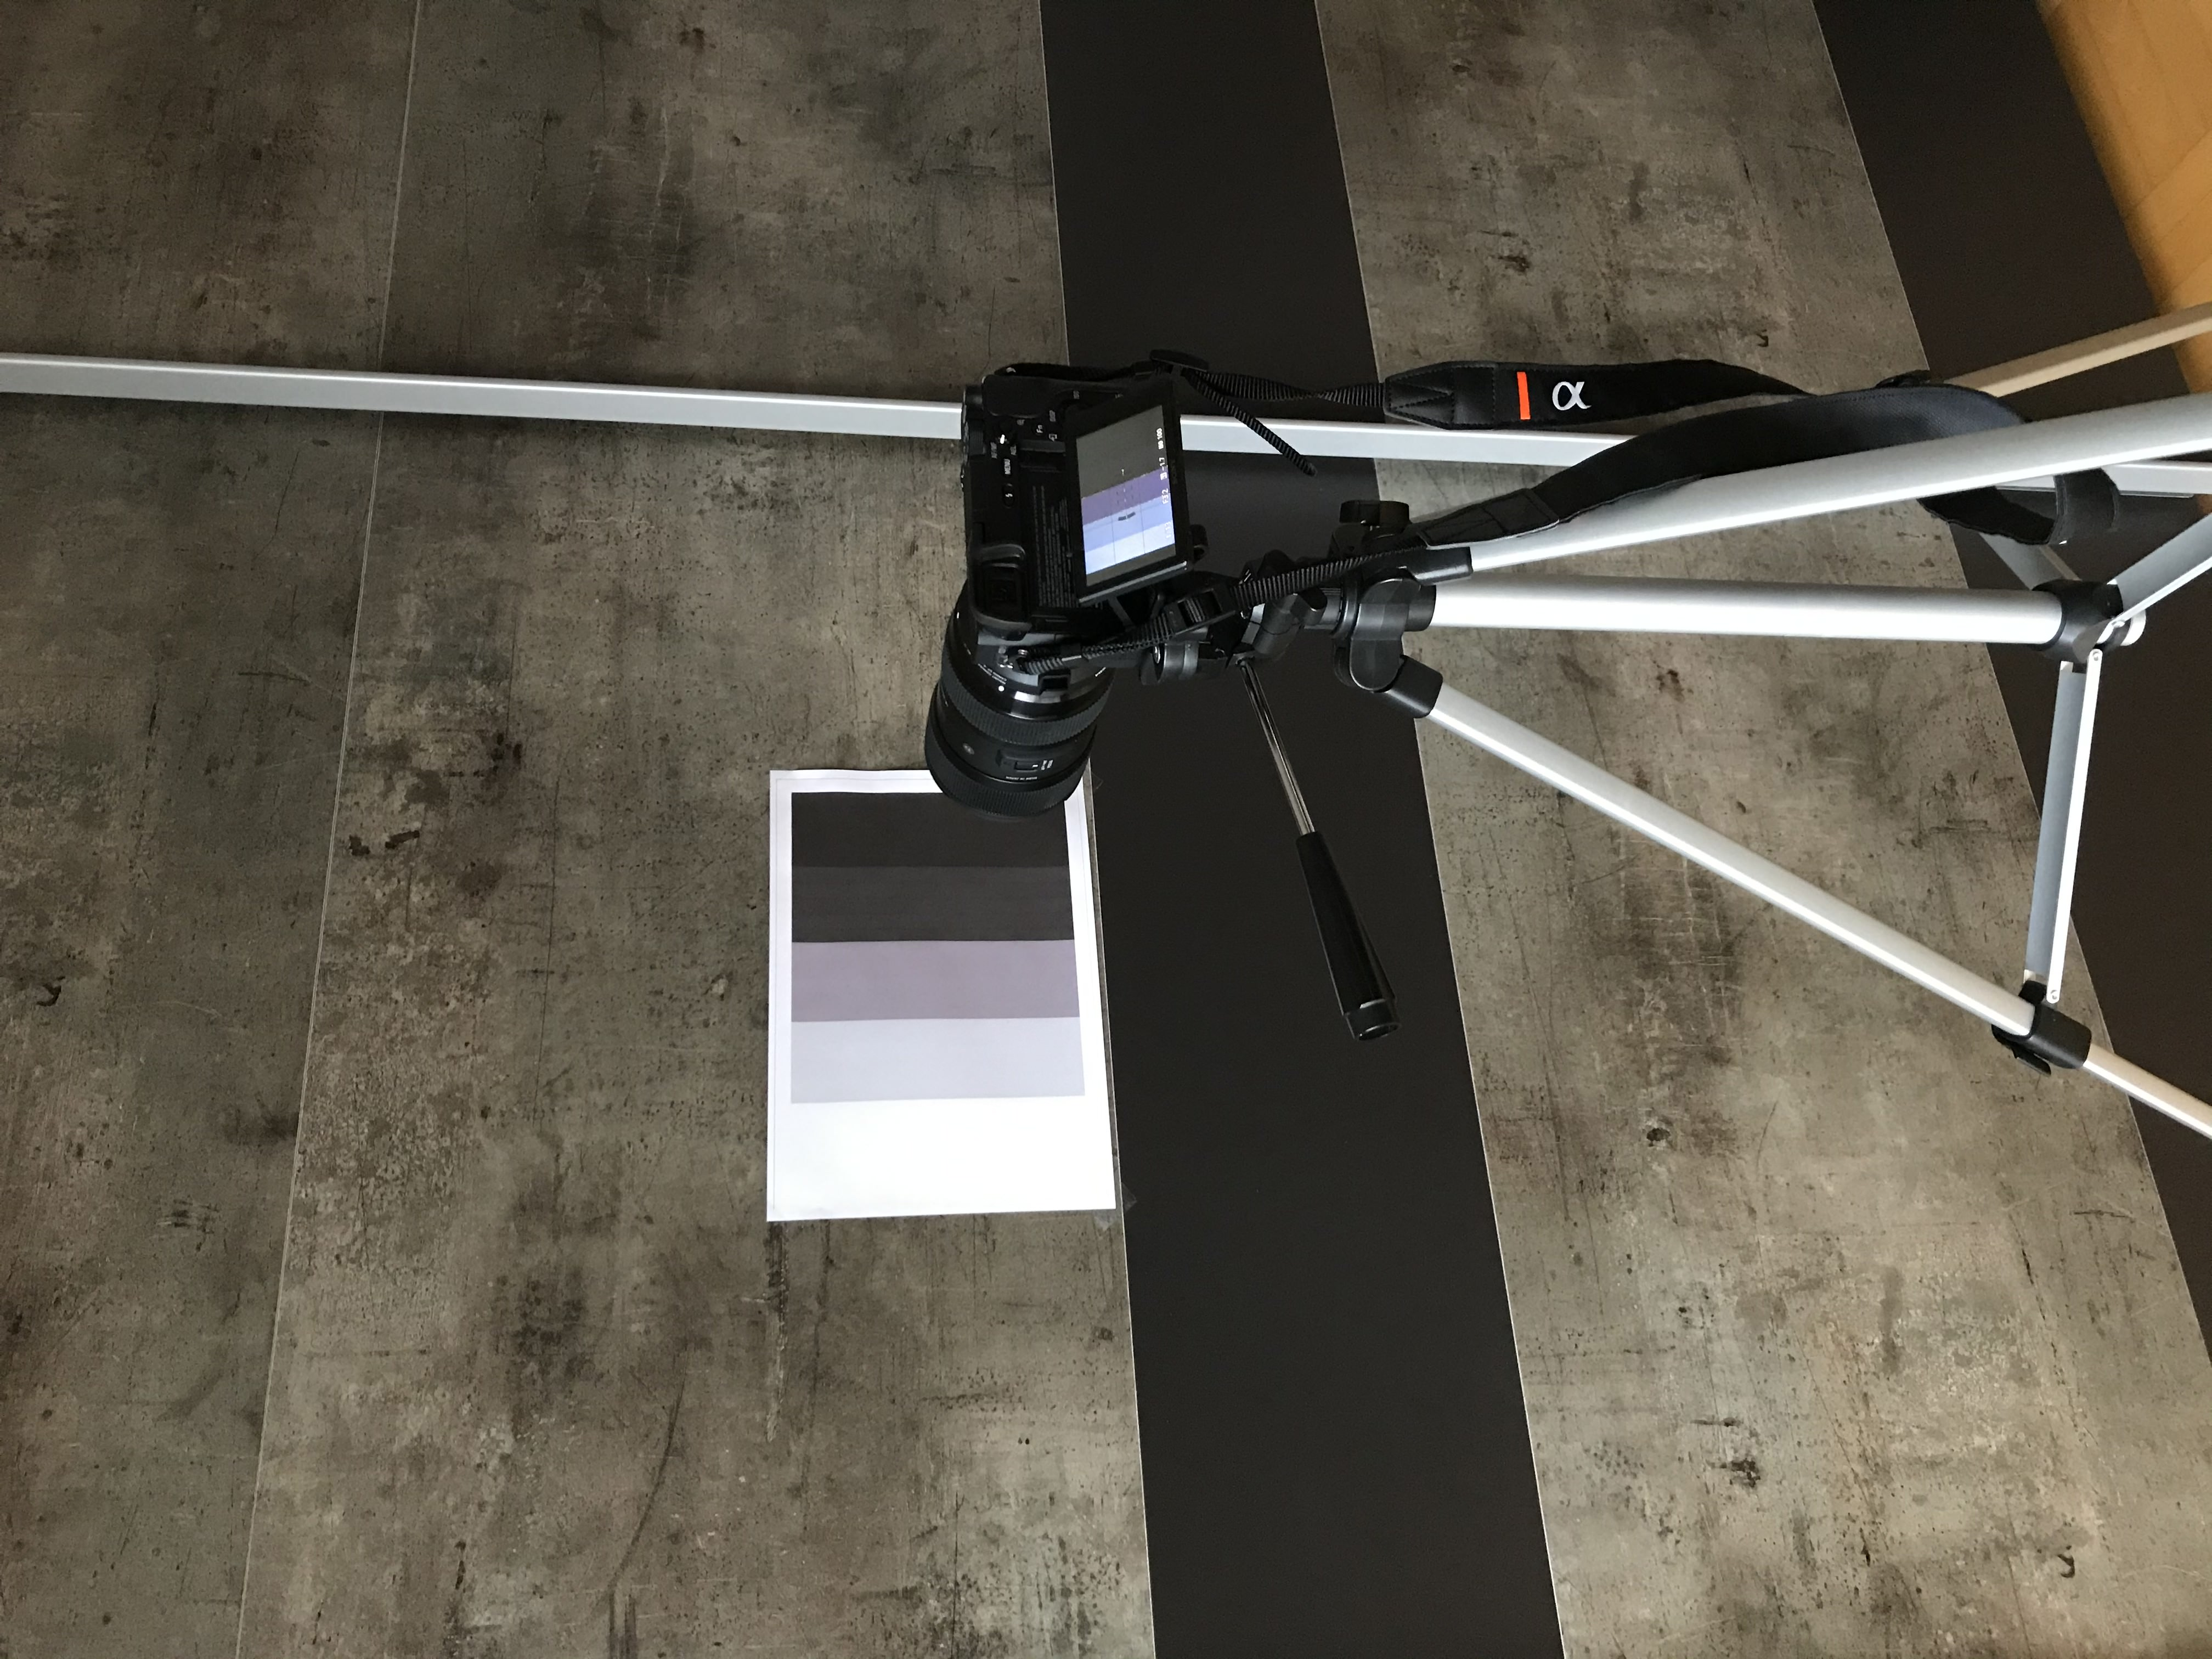
\includegraphics[width=\textwidth, angle=-90, scale=0.8]{media/Versuchsaufbau_Grauwertkeil}
	\caption{Versuchsaufbau}
	\label{fig:VERSUCH_1_AUFBAU}
\end{figure}
\newpage
\section{Messwerte}
\label{chap:VERSUCH_1_MESSWERTE}
Die Aufnahme mit den Einstellungen aus der Tabelle \ref{fig:VERSUCH_1_MESSWERTE_TABELLE} ergab folgendes Bild \ref{fig:VERSUCH_1_MESSWERTE_ORIGINAL}.

\begin{figure}[H]
	\centering\small
	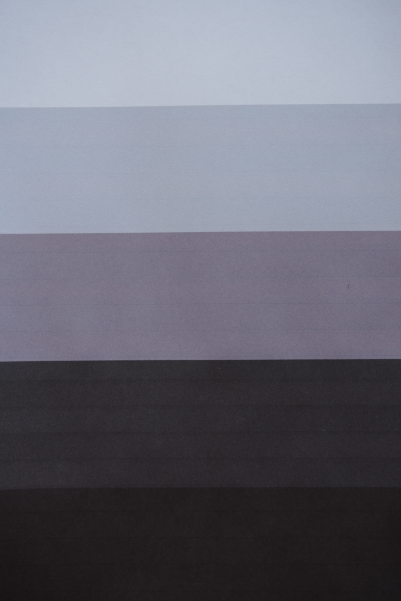
\includegraphics[width=\textwidth, angle=90, scale=0.6]{media/original_versuch1.png}
	\caption{Der Grauwertkeil}
	\label{fig:VERSUCH_1_MESSWERTE_ORIGINAL}
\end{figure}

\begin{table}[H]
\centering\small
\begin{tabular}{|l|l|}
\hline
\textbf{Beschreibung}                & \textbf{Wert} \\ \hline
Frame Width							 & 600			 \\ \hline
Frame Height						 & 400			 \\ \hline
ISO                                  & 100           \\ \hline
Blende                               & f3.2          \\ \hline
Verschlusszeit                       & 1/13          \\ \hline
Manueller Fokus                      & Ja            \\ \hline
Abstand von Objektiv zu Grauwertkeil & 32.5cm        \\ \hline
\end{tabular}
\caption{Einstellungen der Sony A6300}
\label{fig:VERSUCH_1_MESSWERTE_TABELLE}
\end{table}
\newpage
\section{Auswertung}
\label{chap:VERSUCH_1_AUSWERTUNG}
Das Originalbild wird mit der Funktion cv2.cvtcolor in ein Grauwertbild umgewandelt. Mithilfe von Indizierung und Index Slicing wurde das Grauwertbild in fünf Unterbilder unterteilt. 

\begin{figure}[hbt!]
      \centering
      \subfloat[Grauwert 1]{
        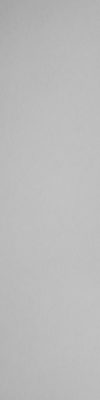
\includegraphics[width=0.08\textwidth]{media/gray1_versuch1.png}\label{fig:f1}}
      \subfloat[Grauwert 2]{
        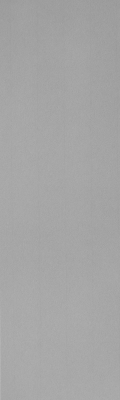
\includegraphics[width=0.08\textwidth]{media/gray2_versuch1.png}\label{fig:f2}}
      \subfloat[Grauwert 3]{
        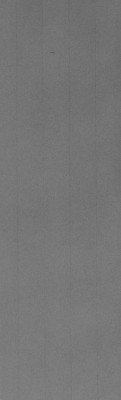
\includegraphics[width=0.08\textwidth]{media/gray3_versuch1.png}\label{fig:f3}}
      \subfloat[Grauwert 4]{
        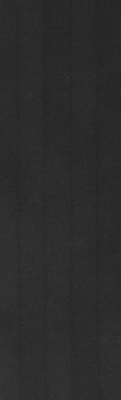
\includegraphics[width=0.08\textwidth]{media/gray4_versuch1.png}\label{fig:f4}}
      \subfloat[Grauwert 5]{
        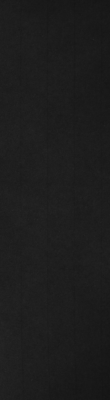
\includegraphics[width=0.08\textwidth]{media/gray5_versuch1.png}\label{fig:f5}}
        \hfill
    \subfloat[Grauwertkeil]{
        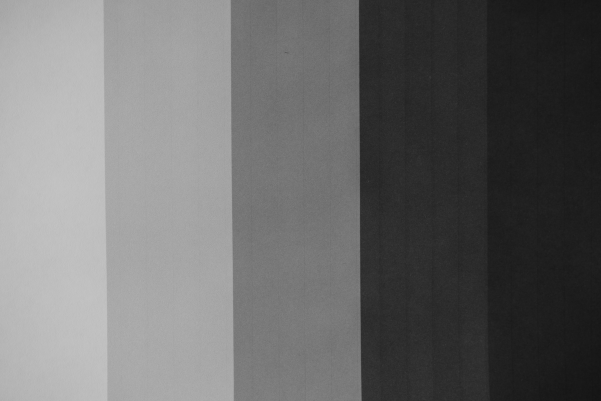
\includegraphics[width=0.4 \textwidth]{media/grauwertkeil_versuch1.png}\label{fig:f6}}
    \caption{Die einzelnen Grauwertsstufen und das zusätzliche Gesamtbild}
    \label{fig:VERSUCH_1_AUSWERTUNG_GRAUWERTKEIL}
\end{figure}

Durch die Funktion cv2.meanStdDev wird die empirische Standardabweichung und der Mittelwert der einzelnen Unterbilder des Grauwertkeils berechnet. Die Ergebnisse der Standardabweichungen und Mittelwerte sehen wir in Abbildung \ref{fig:VERSUCH_1_AUSWERTUNG_BERECHNUNG}.

\begin{figure}[hbt!]
      \centering
      \subfloat[Mittelwert der Grauwerte]{
      	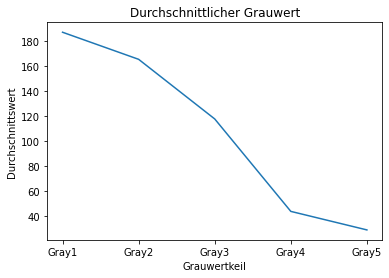
\includegraphics[width=0.45\textwidth]{media/plot_durchschnitt_versuch1.png}\label{fig:f1}}
      \hfill
      \subfloat[Standardabweichung der Grauwerte]{
       	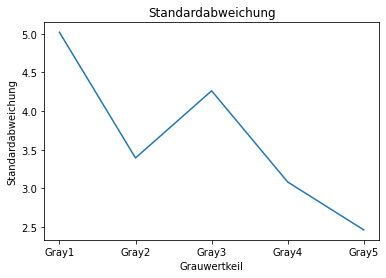
\includegraphics[width=0.45\textwidth]{media/plot_standardabweichung_versuch1.png}\label{fig:f2}}
      \caption{Standardabweichung und Durchschnitt der jeweiligen Grauwerte}
      \label{fig:VERSUCH_1_AUSWERTUNG_BERECHNUNG}
\end{figure}

\section{Interpretation}
\label{chap:VERSUCH_1_INTERPRETATION}
In Abbildung \ref{fig:VERSUCH_1_AUSWERTUNG_GRAUWERTKEIL} ist zu sehen, dass die einzelnen Grauwertkeile unterschiedlich hoch sind, was darauf zurückzuführen ist, dass wir die Array Breite unterschiedlich gewählt haben, um die Stufenränder nicht zu berühren. Die große Standardabweichung bei Gray 1 in \ref{fig:VERSUCH_1_AUSWERTUNG_BERECHNUNG}, könnte daran liegen, dass wir in diesem Bereich am wenigsten Messwerte genommen haben, was das Ergebnis verfälschen könnte.

Zusammenfassend kann man sagen, dass die einzelnen Grauwertstufen eine geringe Standardabweichung aufweisen, was bedeutet, dass fast alle Pixel den gleichen Wert haben.


%
% CHAPTER Versuch 2
%
\chapter{Versuch 2: Aufnahme eines Dunkelbildes}
\label{chap:VERSUCH_2}

\section{Fragestellung, Messprinzip, Aufbau, Messmittel}
\label{chap:VERSUCH_2_FRAGESTELLUNG}
Aufgrund von Fertigungstoleranzen und von spontan entstehenden Ladungsträgerpaaren durch Wärmezufuhr, entsteht ein sogennanter Dunkelstrom. Dieser und das thermische Rauschen der Ausleseelektronik führt dazu, dass jeder Pixel ein leicht unterschiedlicher Nullpunkt hat. Um diesen pixelweisen Offset zu eliminieren, wird in Versuch 2 ein Dunkelbild erstellt. Das Dunkelbild wird von einem Eingabebild subtrahiert und somit bekommt man ein korrigiertes Endbild. Das Dunkelbild haben wir aufgenommen, indem wir das Objektiv komplett abgedeckt haben. In diesem Versuch werden 10 Bilder aufgenommen und dabei pro Pixel ein Mittelwert berechnet. Wenn man alle berechneten Mittelwerte zu einem Bild zusammenfügt, hat man das sogenannte Dunkelbild, das vom Eingabebild subtrahiert werden kann.
\newpage
\section{Messwerte}
\label{chap:VERSUCH_2_MESSWERTE}
In der nachfolgenden Abbildung \ref{fig:VERSUCH_2_MESSWERTE_ORIGINAL} ist eines der aufgenommenen Bilder, wo das Objektiv verdeckt war, dargestellt.

\begin{figure}[H]
	\centering\small
	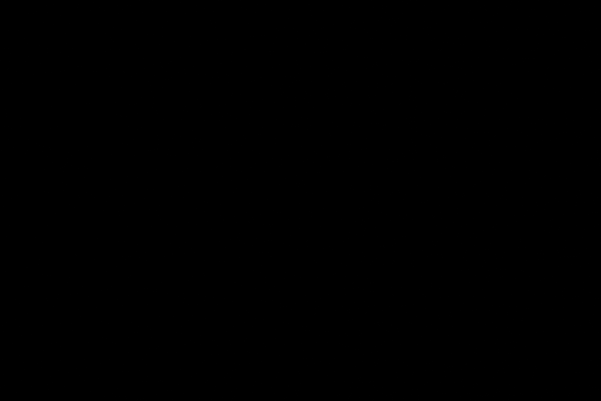
\includegraphics[width=0.5\textwidth]{media/originalBlackImage_versuch2.png}
	\caption{Eins der zehn aufgenommenen Bilder}
	\label{fig:VERSUCH_2_MESSWERTE_ORIGINAL}
\end{figure}

\section{Auswertung}
\label{chap:VERSUCH_2_AUSWERTUNG}
Um das Objektiv abzudecken, haben wir die standard mitgelieferte Schutzkappe verwendet. Dadurch konnten wir ein maximal dunkles Bild erzielen.
Zu aller erst haben wir die 10 aufgenommenen Bilder eingelesen, in ein Grauwertbild umgewandelt und anschließend in ein float image konvertiert. Danach haben wir den pixelweisen Mittelwert berechnet und in einem Ausgabebild gespeichert, welches wir zuvor wieder zurück konvertiert haben als int image. Das Ausgabebild wurde dann mit der Funktion cv2.equalizeHist kontrastmaximiert und zum Schluss vom Grauwertkeilbild subtrahiert. Das konstrastmaximierte Bild ist in Abbildung \ref{fig:VERSUCH_2_MESSWERTE_CONSTRAST} zu sehen.

\begin{figure}[H]
	\centering\small
	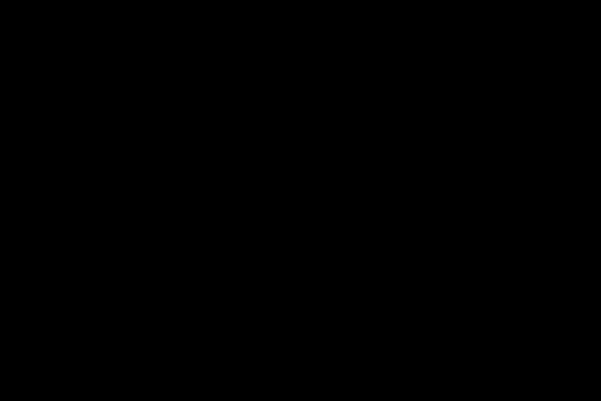
\includegraphics[width=0.5\textwidth]{media/maxContrastBlackImage_versuch2.png}
	\caption{Konstrastmaximiertes Dunkelbild}
	\label{fig:VERSUCH_2_MESSWERTE_CONSTRAST}
\end{figure}

Der korrigierte Grauwertkeil ist in Abbildung \ref{fig:VERSUCH_2_MESSWERTE_CORRECTED} dargestellt.

\begin{figure}[H]
	\centering\small
	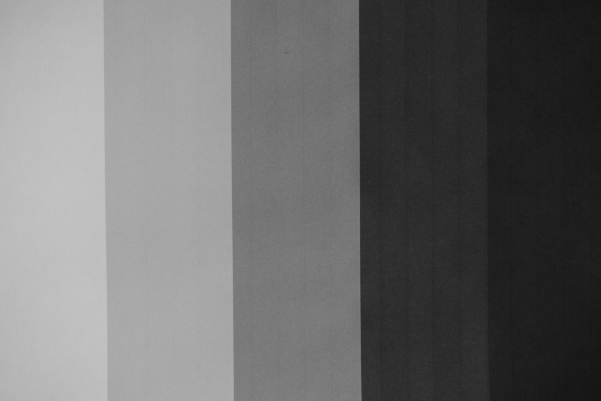
\includegraphics[width=0.5\textwidth]{media/subGrayIntImage_versuch2.png}
	\caption{Korrigierter Grauwertkeil}
	\label{fig:VERSUCH_2_MESSWERTE_CORRECTED}
\end{figure}

\section{Interpretation}
\label{chap:VERSUCH_2_INTERPRETATION}
Da unser korrigierter Grauwertkeil relativ ähnlich, wenn nicht sogar identisch zu unserem Ausgangsbild ist, können wir davon ausgehen, dass unsere verwendete Kamera, so gut wie keine Dunkelströme aufweist und die schwarzen Farben sehr gut aufnimmt. Des weiteren hatten auch unsere Pixel der aufgenommenen zehn Bilder, einen sehr nahen Wert an null, bzw. nur vereinzelte Pixel standen auf eins. Was dementsprechend ein Dunkelbild ergibt, welches kein starken Einfluss auf die Subtraktion des Eingangsbildes hat.
%
% CHAPTER Versuch 3
%
\chapter{Versuch 3: Aufnahme eines Weißbildes}
\label{chap:VERSUCH_3}

\section{Fragestellung, Messprinzip, Aufbau, Messmittel}
\label{chap:VERSUCH_3_FRAGESTELLUNG}
Im dritten Versuch handelt es sich um den Effekt der Vignettierung. Die ungleichmäßige Übertragung der Helligkeit  auf den Sensor, führt zu einer Abdunkelung des Bildes zu den Rändern hin. Zur Kompensation wird deshalb ein Weißbild aufgenommen. Um dieses zu bekommen, wurden zehn Aufnahmen eines weißen Blatt Papiers gemacht. Der Abstand zur Kamera hat sich nicht geändert. Während der Aufnahme der Bilder wurde darauf geachtet, dass der Lichteinfluss auf das Blatt Papier gleichmäßig verteilt ist. Theoretisch bräuchte man für jede Fokuseinstellung ein eigenes Weißbild, dies soll in diesem Versuch aber nicht beachtet werden.
Mithilfe eines Python Skripts wird der Mittelwert jedes einzelnen Pixels berechnet, um damit das thermische Rauschen eliminieren zu können. Von dem errechneten Mittelwertbild wird das Dunkelbild subtrahiert, welches kontrastmaximiert dargestellt werden soll. Das berechnete Bild soll normiert werden, sodass es den Mittelwert 1 erhält und wird anschließend vom korrigierten Eingangsbild dividiert.
\newpage
\section{Messwerte}
\label{chap:VERSUCH_3_MESSWERTE}
In der nachfolgenden Abbildung \ref{fig:VERSUCH_3_MESSWERTE_WHITE} ist eines der aufgenommenen Weißbilder dargestellt.
\begin{figure}[H]
	\centering\small
	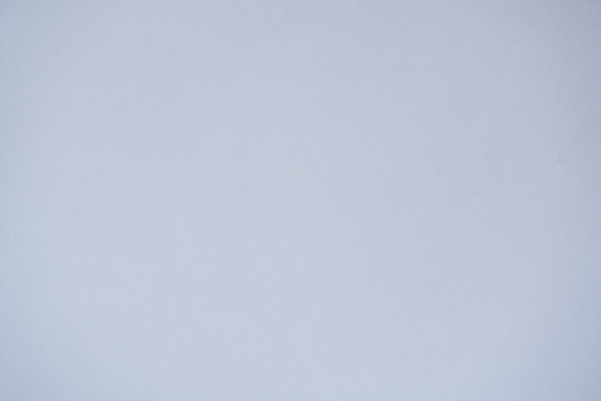
\includegraphics[width=0.5\textwidth]{media/whiteScaled.png}
	\caption{Eins der zehn aufgenommenen Bilder}
	\label{fig:VERSUCH_3_MESSWERTE_WHITE}
\end{figure}
\section{Auswertung}
\label{chap:VERSUCH_3_AUSWERTUNG}
Zuerst wurden die zehn Bilder eingelesen und als Grauwertbilder umgewandelt. Danach wurde der pixelweise Mittelwert berechnet und in einem neuen Bild gespeichert (a), wovon wir dann das kontrastmaximierte Dunkelbild subtrahiert haben. Anschließend wurde das Ergebnis kontrastmaximiert dargestellt. Dies ist in Abbildung  \ref{fig:VERSUCH_3_AUSWERTUNG_WHITEIMG} zu sehen.

\begin{figure}[hbt!]
      \centering
      \subfloat[Pixelweiser Mittelwert der einzelnen Aufnahmen]{
      	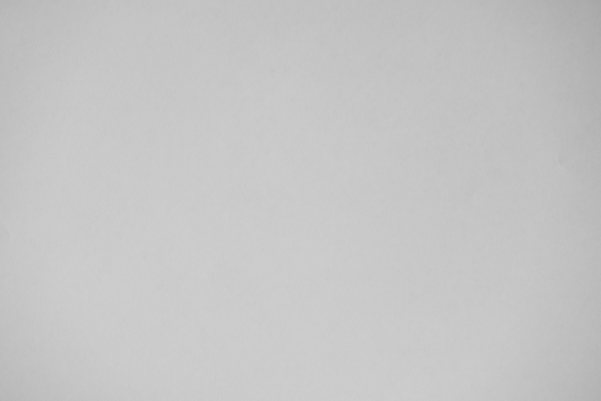
\includegraphics[width=0.45\textwidth]{media/meanWhiteImage.png}\label{fig:f1}}
      \hfill
      \subfloat[Konstrastmaximiertes Weißbild]{
       	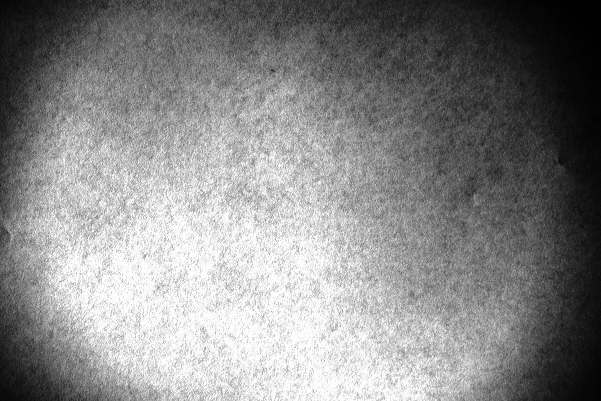
\includegraphics[width=0.45\textwidth]{media/maxContrastWhiteImage.png}\label{fig:f2}}
      \caption{Auswertung Weißbild}
      \label{fig:VERSUCH_3_AUSWERTUNG_WHITEIMG}
\end{figure}

Als nächtes wird das Weißbild normalisiert. Dafür wurden alle Pixel mit dem Mittelwert des ganzen Bildes dividiert. Der Mittelwert des normalisierten Bildes beträgt in unserem Fall 1.0000002. Um das finale Bild aus Abbildung \ref{fig:VERSUCH_3_AUSWERTUNG_NORMAL} zu erhalten, wird das korrigierte Eingangsbild mit dem normalisierten Weißbild dividiert. 

\begin{figure}[H]
	\centering\small
	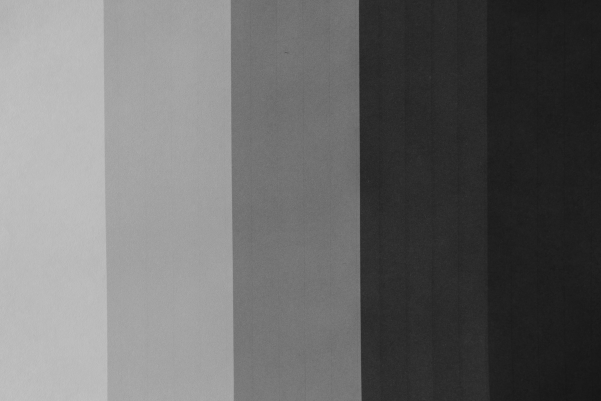
\includegraphics[width=0.5\textwidth]{media/finalImage.png}
	\caption{Das korrigierte Bild aus \ref{fig:VERSUCH_2_MESSWERTE_CORRECTED} dividiert mit dem normalisierten Weißbild}
	\label{fig:VERSUCH_3_AUSWERTUNG_NORMAL}
\end{figure}
\section{Interpretation}
\label{chap:VERSUCH_3_INTERPRETATION}
In dem kontrastmaximierten Weißbild ist die Vignettierung sehr deutlich zu sehen und man erkennt gut an welchen Stellen das Licht nicht gut auf den Sensor übertragen wird. Wie zu erwarten, befindet sich die Vignettierung an den Bildrändern. Bei unserem finalen Bild, erkennt man leider kein großen Unteschied zu dem korrigierten Eingangsbild. Deshalb haben wir die Bilder im Detail analysiert und festgestellt, dass ein Unterschied vorhanden ist, den man aber nicht mit bloßem Auge erkennen kann.

Betrachtet man die Arrays des korrigierten und des finalen Bildes im oberen linken Bereich, wo eine Vignettierung vorhanden ist, sieht man, dass diese im finalen Bild kompensiert wurde und hellere Pixel aufweist. Des Weiteren ist im Bereich der unteren Mitte, wo nur eine schwache Vignettierung vorhanden ist, zu erkennen, dass durch das normalisierte Weißbild die Pixel sich nur schwach verändern. Dieser Vergleich ist in Abbildung \ref{fig:VERSUCH_3_INTERPRETATION_VERGLEICH} dargestellt und Abbildung \ref{fig:VERSUCH_3_INTERPRETATION_BEREICH} verdeutlicht welche Bereiche wir verglichen haben.

\begin{figure}[hbt!]
      \centering
      \subfloat[Korrigiertes Eingangsbild links oben]{
      	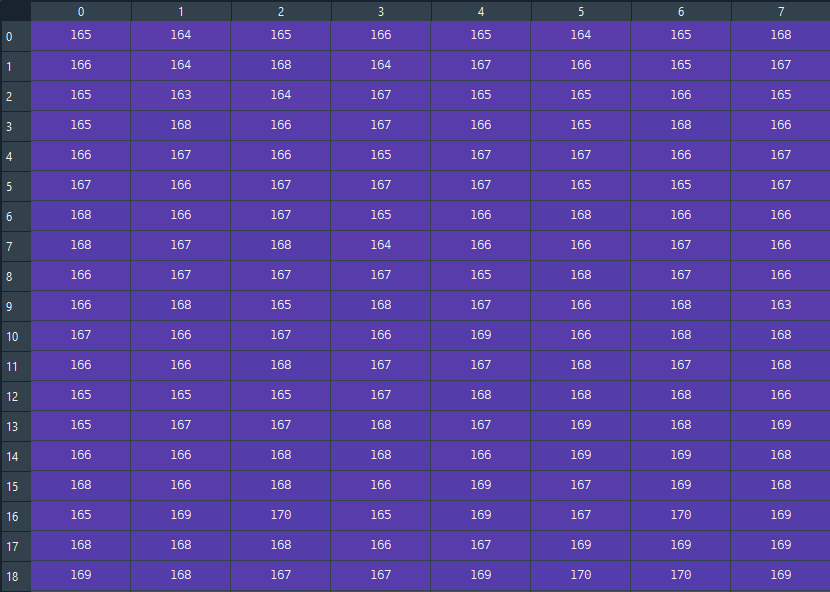
\includegraphics[width=0.45\textwidth]{media/InputImageObenLinks.PNG}\label{fig:f1}}
      \hfill
       \subfloat[Finales Bild aus \ref{fig:VERSUCH_3_AUSWERTUNG_NORMAL} links oben]{
      	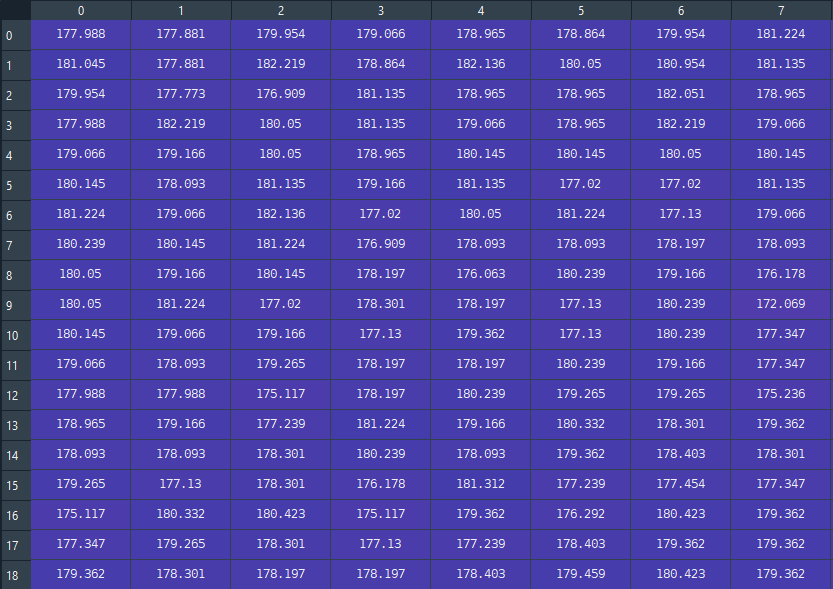
\includegraphics[width=0.45\textwidth]{media/FinalImageObenLinks.PNG}\label{fig:f2}}
      \hfill
      \subfloat[Korrigiertes Eingangsbild unten mitte]{
       	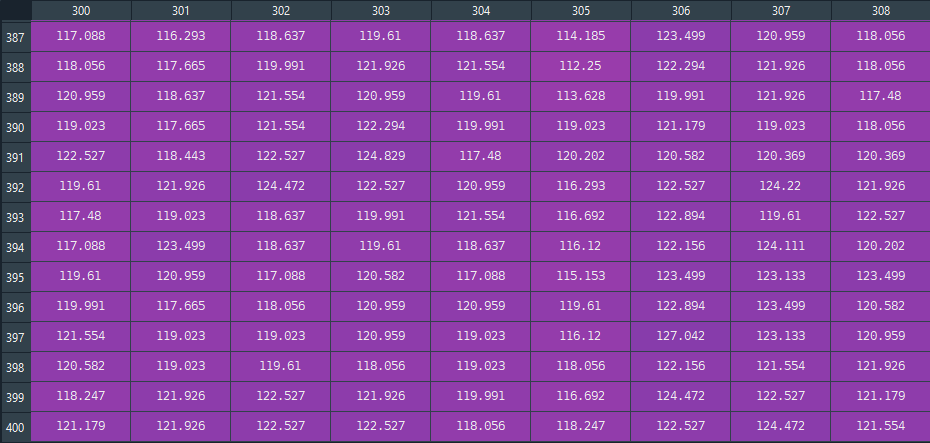
\includegraphics[width=0.45\textwidth]{media/InputImageUntenMitte.PNG}\label{fig:f3}}
       \subfloat[Finales Bild aus \ref{fig:VERSUCH_3_AUSWERTUNG_NORMAL} unten mitte]{
      \hfill
      	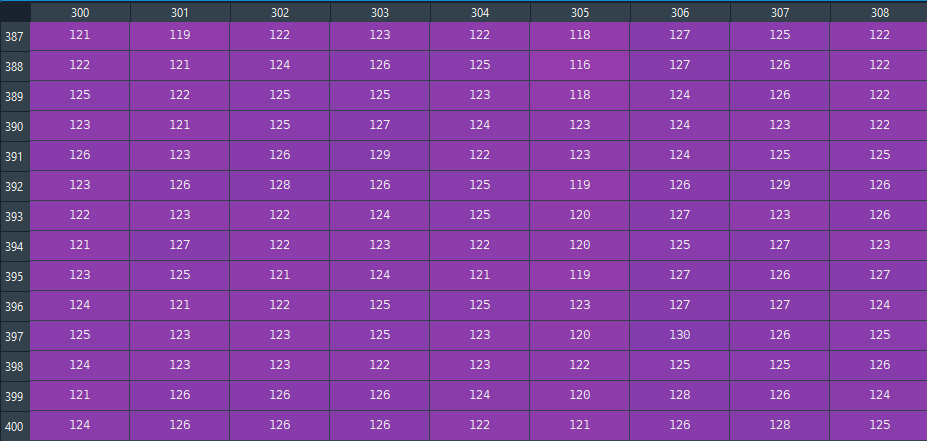
\includegraphics[width=0.45\textwidth]{media/FinalImageUntenMitte.PNG}\label{fig:f4}}
      \caption{Auszüge der Arrays aus dem Python Skript}
      \label{fig:VERSUCH_3_INTERPRETATION_VERGLEICH}
\end{figure}

\begin{figure}[H]
	\centering\small
	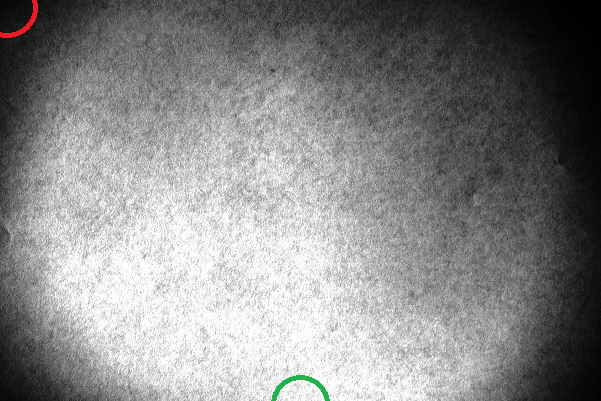
\includegraphics[width=0.5\textwidth]{media/maxContrastWhiteImageEdited.png}
	\caption{Analysierte Bereiche in einem roten und grünen Kreis dargestellt}
	\label{fig:VERSUCH_3_INTERPRETATION_BEREICH}
\end{figure}

%
% CHAPTER Versuch 4
%
\chapter{Versuch 4: Pixelfehler}
\label{chap:VERSUCH_4}

\section{Fragestellung, Messprinzip, Aufbau, Messmittel}
\label{chap:VERSUCH_4_FRAGESTELLUNG}
Im letzten Aufgabenteil wird das Dunkel- und Weißbild auf Funktionsuntüchtige Pixel untersucht. Es gibt verschiedene Arten von funktionsuntüchtigen Pixel, wie z.B. dead, hot und stuck pixel. Dead Pixel bleiben immer auf dem niedrigsten Wert stecken und lassen sich sehr gut auf einem Weißbild identifizieren. Stuck pixel hingegend bleiben immer auf dem Maximalwert und hot pixel gehen bei längerer Belichtungszeit in die Sättigung. Beide können sehr gut auf einem Dunkelbild erkannt werden. Am Schluss wird das finale Bild anhand des Mittelwertes und der Standardabweichung erneut, wie im ersten Versuch, ausgewertet.
\newpage
\section{Messwerte}
\label{chap:VERSUCH_4_MESSWERTE}
In den nachfolgenden Abbildungen, ist die Untersuchung auf funktionsuntüchtige Pixel dargestellt.	 
\begin{figure}[H]
	\centering\small
	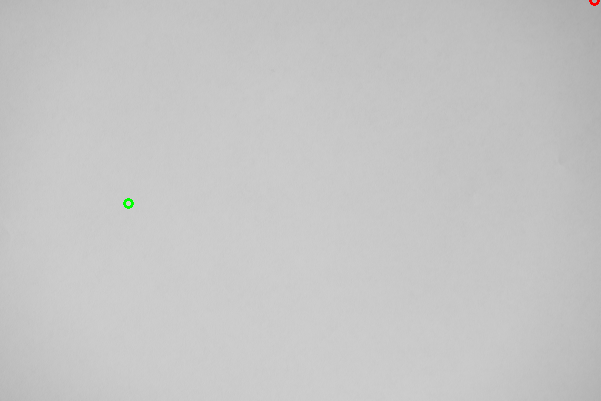
\includegraphics[width=0.7\textwidth]{media/circleWhiteImage.png}
	\caption{Untersuchung Weißbild}
	\label{fig:VERSUCH_4_MESSWERTE_WEISSBILD}
\end{figure}

\begin{figure}[H]
	\centering\small
	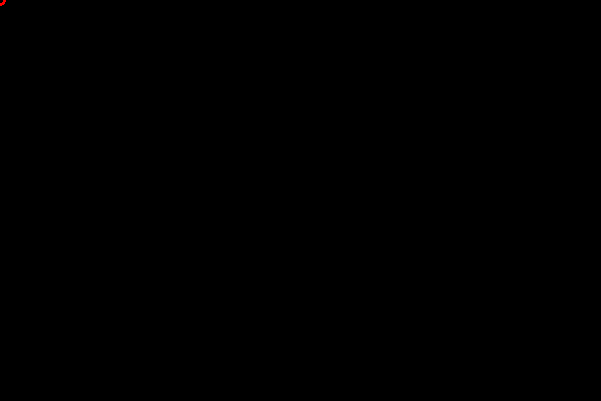
\includegraphics[width=0.7\textwidth]{media/circleBlackImage.png}
	\caption{Untersuchung Weißbild}
	\label{fig:VERSUCH_4_MESSWERTE_DUNKELBILD}
\end{figure}
\section{Auswertung}
\label{chap:VERSUCH_4_AUSWERTUNG}

In Abbildung \ref{fig:VERSUCH_4_MESSWERTE_WEISSBILD} wird das Weißbild auf funktionsuntüchtige Pixel untersucht. Mithilfe unseres Python Skripts haben wir den höchsten und niedrigsten Werte mit verschiedenen Farben eingekreist. Der grüne Kreis stellt den höchsten Wert dar, während der rote den niedrigsten Wert umkreist.

In Abbildung \ref{fig:VERSUCH_4_MESSWERTE_DUNKELBILD} wird das Dunkelbild auf funktionsuntüchtige Pixel untersucht, wobei hier der rote Kreis den grünen überdeckt. Das ist darauf zurückzuführen, dass das Dunkelbild ein Array aus Nullen ist und wir standardmäßig die Kreise auf die Koordinaten (0,0) gesetzt haben.

Die Werte dieser auffäligen Pixel werden in Tabelle \ref{fig:VERSUCH_4_AUSWERTUNG_TABELLE} aufgelistet.

\begin{table}[H]
\centering\small
\begin{tabular}{|l|l|}
\hline
\textbf{Beschreibung}               & \textbf{Wert} \\ \hline
Höchster Wert im Dunkelbild    & 0                     \\ \hline
Niedrigster Wert im Dunkelbild & 0                     \\ \hline
Höchster Wert im Weißbild       & 206                 \\ \hline
Niedrigster Wert im Weißbild    & 166                 \\ \hline
\end{tabular}
\caption{Werte der eingekreisten Pixel}
\label{fig:VERSUCH_4_AUSWERTUNG_TABELLE}
\end{table}

In Abbildung \ref{fig:VERSUCH_4_AUSWERTUNG_BERECHNUNG} wird das finale Bild \ref{fig:VERSUCH_3_AUSWERTUNG_NORMAL} anhand des Mittelwerts und der Standardabweichung ausgewertet.

\begin{figure}[hbt!]
      \centering
      \subfloat[Mittelwert der Grauwerte]{
      	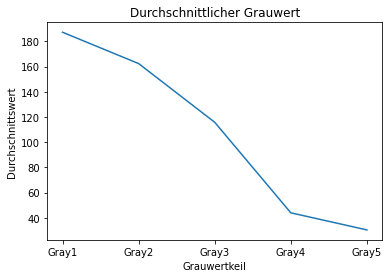
\includegraphics[width=0.45\textwidth]{media/plot_durchschnitt_final.png}\label{fig:f1}}
      \hfill
      \subfloat[Standardabweichung der Grauwerte]{
       	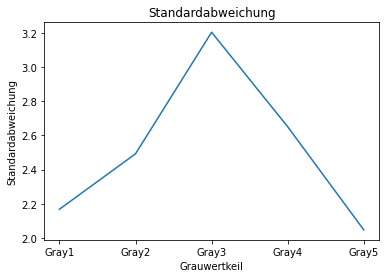
\includegraphics[width=0.45\textwidth]{media/plot_standardabweichung_final.png}\label{fig:f2}}
      \caption{Standardabweichung und Durchschnitt der jeweiligen Grauwerte}
      \label{fig:VERSUCH_4_AUSWERTUNG_BERECHNUNG}
\end{figure}

\section{Interpretation}
\label{chap:VERSUCH_4_INTERPRETATION}
Da im Dunkelbild der höchste Pixel den Wert Null hat, ist daraus zu schließen, dass es sich hierbei nicht um hot oder stuck pixels handelt. Im Weißbild hat der niedrigste Pixel den Wert 166, was darauf hindeutet, dass es sich hier nicht um ein dead pixel handelt. Aus den zwei Erkenntnissen, schließen wir daraus, das unsere verwendete Kamera keine funktionsuntüchtigen Pixels besitzt.

Es ist zu sehen, dass die Standardabweichung generell etwas niedriger ausfällt, als im ersten Versuch. Dabei sticht deutlich der erste Grauwertkeil heraus, da die Standardabweichung von 5 auf 2.2 geschrumpft ist. Dass ist darauf zurückzuführen, dass es sich bei dem ersten Grauwertkeil um den weißen Teil handelt und die Vignettierung dabei aufgehoben wird.

%
% CHAPTER Anhang
%
\renewcommand\thesection{A.\arabic{section}}
\renewcommand\thesubsection{\thesection.\arabic{subsection}}

\chapter*{Anhang}
\label{chap:APPENDIX}
\addcontentsline{toc}{chapter}{Anhang}
%\setcounter{chapter}{0}
\addtocounter{chapter}{1}
\setcounter{section}{0}

\section{Quellcode}
\label{chap:APPENDIX_SOURCECODE}

\subsection{Quellcode Versuch 1}
\label{chap:APPENDIX_SOURCECODE_V1}	
\lstinputlisting[style=PYTHON, frame=single, caption=Skript Versuch 1, captionpos=b, label=lst:APPENDIX_SOURCECODE_PLOT]{code/versuch1_1.py}
\newpage
\subsection{Quellcode Versuch 2}
\label{chap:APPENDIX_SOURCECODE_V2}
\lstinputlisting[style=PYTHON, frame=single, caption=Skript Versuch 2, captionpos=b, label=lst:APPENDIX_SOURCECODE_PLOT]{code/versuch2_2.py}
\newpage
\subsection{Quellcode Versuch 3}
\label{chap:APPENDIX_SOURCECODE_V3}
\lstinputlisting[style=PYTHON, frame=single, caption=Skript Versuch 3, captionpos=b, label=lst:APPENDIX_SOURCECODE_PLOT]{code/Versuch2_3.py}
\lstinputlisting[style=PYTHON, frame=single, caption=Skript Versuch 3b, captionpos=b, label=lst:APPENDIX_SOURCECODE_PLOT]{code/Versuch2_3b.py}
\newpage
\subsection{Quellcode Versuch 4}
\label{chap:APPENDIX_SOURCECODE_V4}
\lstinputlisting[style=PYTHON, frame=single, caption=Skript Versuch 4, captionpos=b, label=lst:APPENDIX_SOURCECODE_PLOT]{code/Versuch2_4.py}
\lstinputlisting[style=PYTHON, frame=single, caption=Skript Versuch 4b, captionpos=b, label=lst:APPENDIX_SOURCECODE_PLOT]{code/Versuch2_4b.py}

\end{document}
%------------------------------------
% ╔═╗╔╗╔╔╦╗  ╔╦╗╔═╗╔═╗╦ ╦╔╦╗╔═╗╔╗╔╔╦╗
% ║╣ ║║║ ║║   ║║║ ║║  ║ ║║║║║╣ ║║║ ║
% ╚═╝╝╚╝═╩╝  ═╩╝╚═╝╚═╝╚═╝╩ ╩╚═╝╝╚╝ ╩
%------------------------------------